\newpage
\section{Prac 5 - ALU}
\label{sec:Prac5}
\subsection{Overview}
An arithmetic logic unit (ALU) is a digital building block which can perform a variety of arithmetic, logical and bit shift operations. It is the base building block of a central processing unit and operates on integer binary numbers. The unit has both data and control signals. A basic ALU has two parallel input data busses (A) and (B) and one parallel output data bus (Y). It also has a parallel bus (F) which takes in an opcode or binary value which selects a specific arithmetic, logical or shift operation to be performed by the ALU on the two inputs A and B, it may also have a status output bus S which gives more information about the previous operation.
\begin{figure}[H]
\centering
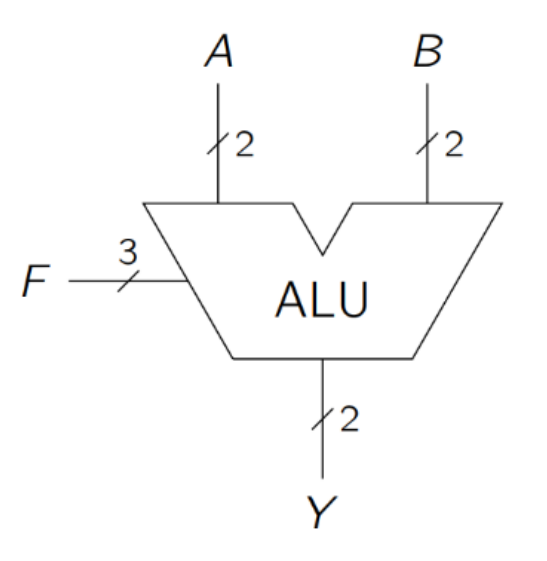
\includegraphics[width=0.35\columnwidth]{Figures/ALU}
\caption{An Example of a simple ALU with a 2-bit wide data bus}
\label{fig:ALU}
\end{figure}

\subsection{Pre-Practical Requirements}
\begin{itemize}
    \item Logisim
    \item Latex
\end{itemize}

\subsection{Deliverables}
\begin{itemize}
    \item Design the ALU using logical building blocks. Explain each step in your report. (30) \footnote{This is not a technical report as the one expected in practical 2. However, each building blocks must be represented in a figure, the functionality and the role of each building block in the bigger system must be explained.}
    \item Simulate your design in Logisim. Clearly label all inputs, outputs etc. Export a jpeg of the circuit and include it in your report. (10)
    \item Marks will be deducted for incomplete or untidy reports.
\end{itemize}


\subsection{Further Instructions}
You are required to design and implement a 2-bit wide ALU with a 3 bit opcode, as follows:
% Please add the following required packages to your document preamble:
% \usepackage{graphicx}
\begin{table}[H]
\centering
\caption{Three bit opcode and equivalent operation}
\label{tbl:Opcodes}
\begin{tabular}{|c|c|c|c|c|}
\hline
\multicolumn{3}{|c|}{\textbf{Opcode}} & \multicolumn{2}{c|}{\textbf{Function}} \\ \hline
$F_2$ & $F_1$ & $F_0$ & \multicolumn{2}{c|}{F} \\ \hline
0 & 0 & 0 & A+B & Addition \\ \hline
0 & 0 & 1 & A-B & Subtration \\ \hline
0 & 1 & 0 & A+1 & Increment \\ \hline
0 & 1 & 1 & A-1 & Decrement \\ \hline
1 & 0 & 0 & A $\times$ 2 & Multiply by 2 \\ \hline
1 & 0 & 1 & A $\div$ 2 & Divide by 2 \\ \hline
1 & 1 & 0 & A $\wedge$ B & Bit-wise AND \\ \hline
1 & 1 & 1 & A $\vee$ B & Bit-wise OR \\ \hline
\end{tabular}%
\end{table}